\section{The Problem as a Graph}\label{sec:asgraph-\myInitials}

% Discuss here how instances of that problem can be expressed as a graph.

We can formalize the above problem as a complex, heterogeneous network. With the following structure:

\begin{center}
    \parbox[t]{2.4in}{
        \raggedright%
        \textbf{\textit{Node Types :}}
        \begin{enumerate}[topsep=0pt,itemsep=-2pt,leftmargin=13pt]
            \item Airport
            \item Seaport
            \item Rail Station
        \end{enumerate}
    }%
    \parbox[t]{2.4in}{
        \raggedright%
        \textbf{\textit{Edge Properties :}}
        \begin{enumerate}[topsep=0pt,itemsep=-2pt,leftmargin=13pt]
            \item Direction
            \item Transition Probability ($p_1...p_k$)
            \item Distance
            \item Travel Time
        \end{enumerate}
    }
\end{center}

\begin{figure}
    \centering
    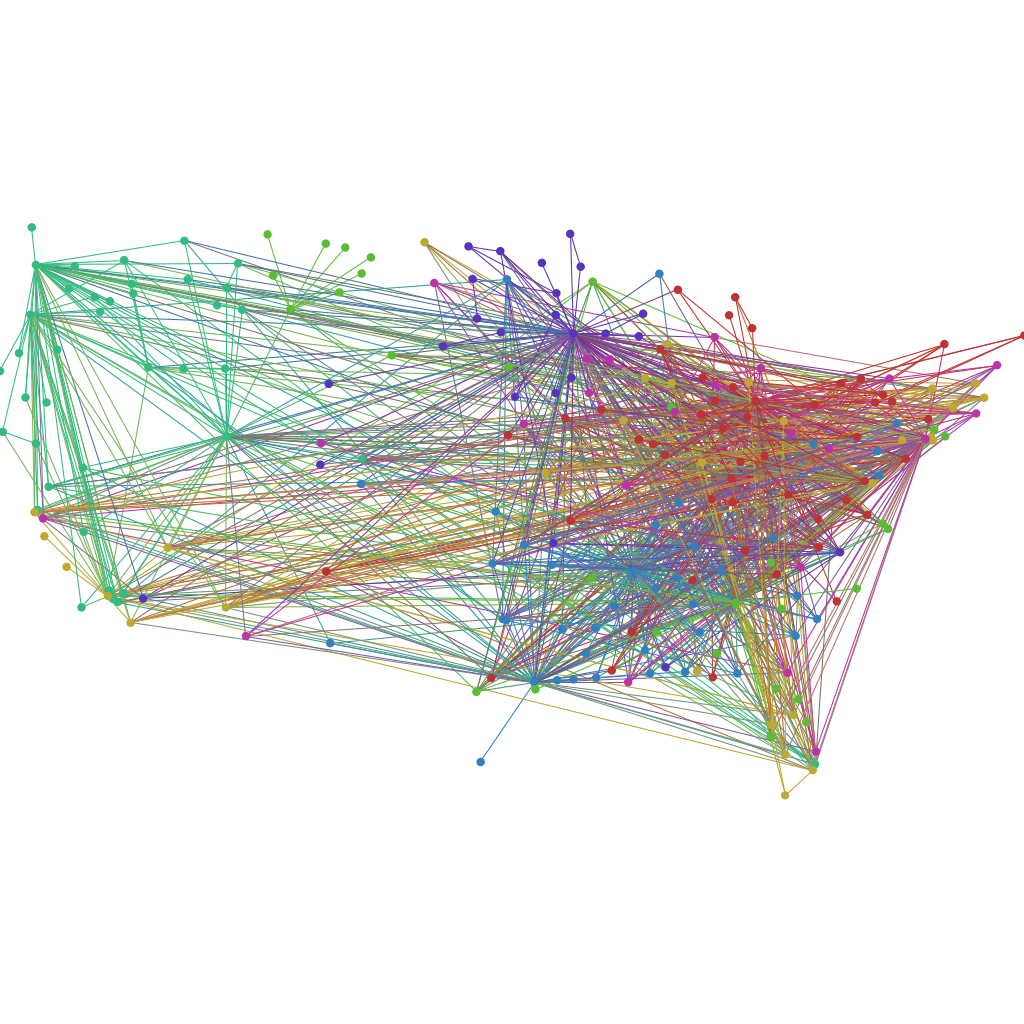
\includegraphics[width=1.0\textwidth]{figures-RW/usairport_base.png}
    \caption{US Domestic Airport Network\cite{stanford_dhs}}
    \label{fig:us_domestic}
\end{figure}

\newpage
Figure \ref{fig:us_domestic} shows a network containing only nodes of type \textit{airport}, with edges weighted and colored by the frequency of travel between two airports.

